
\section{INTRODUCTION}
Bayesian inference and prediction in large complex models, as in 
deep neural networks or stochastic processes, remains as an elusive problem \cite{blei2017variational,insua2012bayesian,alquier2020approximate}.
%
%as in 
%Accurate and efficient uncertainty estimation is becoming increasingly relevant in the Machine Learning community. As current models, such as those grounded in deep learning \cite{SCHMIDHUBER201585}, become more and more complex, traditional uncertainty estimation techniques become obsolete, thus the growing interest in developing newer approximation frameworks.
%
%One of the most popular and flexible paradigms to perform uncertainty estimation is provided by Bayesian statistics \cite{gelmanbda04}. Consider a joint probability model of latent variables and parameters $z$ and observations $x$,
%$$
%p(x,z) = p(z)p(x|z). 
%$$
%Under the Bayesian paradigm, the latent variables govern the distribution of the observed data. A Bayesian probabilistic model draws the latent variables or parameters from some prior distribution $p(z)$ and relates them to the observations via the likelihood probability $p(x|z)$. The machine learning and artificial intelligence communities are pervaded by models that can be expressed naturally through a joint model. Variational autoencoders (VAE) \cite{kingma2013auto} or  hidden Markov models (HMM) \cite{rabiner1989tutorial} are two relevant examples. 
%
%To perform Bayesian inference, we need to condition on the data to compute the posterior distribution, which we can be used to get uncertainty estimates. In complex models, this distribution 
Variational approximations (e.g., Automatic Differentiation Variational Inference (ADVI) \cite{kucukelbir2017automatic}) tend to be biased and 
underestimate uncertainty \cite{riquelme2018failure}. 
On the other hand, depending on the target distribution,
%is frequently intractable and requires approximations, such as Monte Carlo methods (e.g.,
Markov Chain Monte Carlo (MCMC) \cite{andrieu2010particle} 
methods, such 
as Hamiltonian Monte Carlo (HMC) \cite{neal2011mcmc}),   
tend to be exceedingly slow  \cite{van2018simple} {\bf in large scale settings with large amounts of data points and/or  parameters}. For such reason, over the recent years, there has been an increasing interest in developing more efficient posterior approximations \cite{nalisnick2016approximate,salimans2015markov,tran2015variational} and inference techniques that aim to be as general and flexible as possible {\bf so that they can be easily used easily with any probabilistic model} \cite{wood2014new, ge2018t}.

It is well known that the performance of a sampling method depends
heavily on the parameterization used \cite{papaspiliopoulos2007general}. This work proposes
a framework to automatically tune the parameters of a 
MCMC sampler {\bf  aimed at adapting the shape of the posterior, thus boosting Bayesian inference efficiency. 
 We deal with the case in which the latent variables or parameters are continuous. Our framework can be regarded as well as a principled way to enhance the flexibility of the variational posterior approximation, in search of an optimally tuned MCMC sampler.}
Hence the proposed name of {\em variationally inferred sampler} (VIS).


{ \bf

The idea of preconditioning the posterior distribution to speed up the mixing time of a MCMC sampler has been explored recently in \cite{hoffmanneutra} and \cite{PhysRevLett.121.260601}, where a parameterization is learnt before sampling via HMC. Both papers extend seminal work in \cite{parno2014transport} by learning an efficient and expressive deep, non-linear transformation instead of a polynomial regression. However, they do not account for tuning the parameters of the sampler as introduced in Section \ref{sec:main}, where a fully, end to end differentiable sampling scheme is proposed.

The work of \cite{rezende2015variational} introduced a general
framework for constructing more flexible variational distributions, called normalizing flows. These transformations are one of the main techniques to improve the flexibility of current variational inference (VI) approaches and have recently pervaded the approximate Bayesian inference
literature with developments such as continuous-time normalizing flows \cite{chen2018continuoustime} (which extend an initial simple variational posterior with a discretization of Langevin dynamics) or the Householder flow for mixtures of Gaussian distributions \cite{LIU201943}. However, they require a generative adversarial network (GAN) \cite{goodfellow2014generative} to learn the posterior,
which can be unstable in high-dimensional spaces. We overcome this with our novel formulation; moreover, our framework is also compatible with different optimizers, not only those derived from Langevin dynamics \cite{10.5555/3122009.3208015}. Other recent proposals create more flexible variational posteriors are based on implicit approaches typically requiring a GAN like \cite{huszar2017variational}, UIVI \cite{pmlr-v89-titsias19a} or SIVI \cite{yin2018semi}. Our variational approximation is also implicit but uses a sampling algorithm to drive the evolution of the density, combined with a Dirac delta approximation to derive an efficient variational approximation, as reported through extensive experiments in Section \ref{sec:exps}.

Closely related to our framework is \cite{hoffman2017learning}, where a VAE is learned using HMC. We use a similar compound distribution as the variational approximation, yet 
our approach allows for embedding any \emph{stochastic gradient} MCMC, %(SG-MCMC) sampler parameterized as $Q_{\eta, T}(z|z_0)$, where $z_0$ is the initial sample, $\eta$ the sampler hyperparameters and $T$ denotes the number of iterations.
facilitating as well the tuning of sampler parameters via gradient descent.
Our work also relates to the recent idea of 
sampler amortization \cite{feng2017learning}. 
A common problem with these approaches is that they incur in an additional error, the amortization gap \cite{cremer2018inference}; we alleviate it 
by evolving a set of particles through a stochastic process in the latent space after learning a good initial distribution,
so that %. Hence, the bias generated by 
the initial approximation bias is significantly reduced.
%after several process iterations % of the process.
A recent related article is \cite{pmlr-v97-ruiz19a}
which defines as well a compound distribution. 
However, our focus is on an efficient approximation using the reverse KL divergence, %the standard and well understood divergence used in variational inference, 
which allows for tuning sampler parameters and achieving superior results. Apart from optimizing such divergence, % (better studied than the divergence  use),
the main point is that we can compute gradients wrt sampler parameters %$\eta$ 
(Section \ref{sec:tuning}), whereas in \cite{pmlr-v97-ruiz19a} the authors only consider a parameterless sampler: % $Q_T(z|z_0)$:
our framework allows for greater flexibility, helping the user
in tuning  sampler hyperparameters.
In the Coupled Variational Bayes (CVB) \cite{dai2018coupled} approach,
optimization is in the dual space whereas
we  optimize the standard
evidence lower bound (ELBO). Note that even if the optimization was exact the solutions would coincide, it is not clear yet what happens in the truncated optimization case,% (finite $T$), 
other than performing empirical experiments on given datasets. We thus feel that there is room for implicit methods that perform optimization in the primal space 
(besides they are easier to implement). Moreover,
the previous \emph{dual optimization} approach requires the use of an additional neural network, see the CVB paper or \cite{fang2019implicit}. This adds a large amount of parameters and another architecture decision. With VIS we do not need to introduce an auxiliary network, since we perform a "non-parametric" approach by backpropagating instead through 
several iterations of SGLD. %Thus, the only parameters introduced are the sampler hyperparameters (the step-size in the SGLD case).
Moreover, the lack of an auxiliary network simplifies the design choices.
}


%If we consider a probabilistic program to define a distribution $p(x, z)$, where $x$ are observations and $z$  denote both latent variables and parameters, then we are typically interested in answering queries involving the posterior $p(z | x)$. 

{\bf Thus, our contributions include first, a flexible and consistent variational approximation to the posterior,
embedding an initial variational approximation within a stochastic process;} %, together with 
an analysis of its key properties; %(Section \ref{sec:main}); 
    the provision of several strategies for the ELBO
    optimization using the previous 
    approximation; and, finally, 
    an illustration of its power through relevant complex examples.
    %\item An alternative ELBO function objective formulation, which is a variant of the original one when this new variational approximation is adopted. %(Section \ref{sec:rewriting}).
    %\item A specialization to the case of Bayesian inference in state-space models.% (Section \ref{sec:ss}).
    %\item Variance reduction and reparameterization via delayed sampling to accelerate the sampling process.
    %\item Guide generation (special structure in the warping flow).


 


%BMAML: only SVGD, focus on multiple tasks, custom losses.

\section{BACKGROUND}
%\section{Background}
Consider a probabilistic model $p(x|z)$ and a prior distribution $p(z)$, where $x$ denotes the observations and $z \in \mathbb{R}^d$ the unobserved latent variables or parameters, depending on the context. Whenever necessary for disambiguation
purposes, we shall distinguish between $z$ for latent variables and $\theta$ for parameters. Our interest is in performing inference regarding the unobserved $z$ by approximating its posterior distribution
$$
p(z| x) = \frac{ p(z)p(x| z) }{ \int p(z)p(x| z) dz} = %\frac{ p(z)p(x| z) }{ p(x) } = 
\frac{p(x, z)}{p(x)}.
$$
The integral assessing the evidence $p(x) = \int p(z)p(x| z) dz$ is typically intractable. %; no general explicit expressions of the posterior are available. 
Thus, several techniques have been proposed to perform approximate posterior inference {\bf \cite{alquier2020approximate}}.



\iffalse
A probabilistic program defines a probabilistic model $p(x, z)$ that factorizes as
$$
p(x, z) = p(x | z) \prod_{i=1}^n p(z_i | z_{<i}),
$$
where $n$ is the number of latent variables. The previous notation is convenient since it resembles the structure of a generic probabilistic model to sample from $p(x, z)$:
\begin{align*}
    z_1 &\sim p(z_1) \\
    z_2 &\sim p(z_2 | z_{<2}) = p(z_2 | z_1) \\
    &\ldots \\
    z_n &\sim p(z_n | z_{<n}) \\
    x &\sim p(x | z) \\
    \mbox{\texttt{o}}&\mbox{\texttt{bserve }}x,
\end{align*}
where we have $n+1$ sampling statements and then we can condition
 on some observed data. Note that the last factor $p(x|z)$ could be also further factorized. This formulation is sufficiently flexible to describe numerous models typically used in the Machine Learning community, such as the Hidden Markov Model, whose joint probability can be expressed as
$$
p(x, z)
= p(x | z) \prod_{i=1}^\tau p(z_i | z_{i-1}) = \prod_{i=1}^\tau p(x_i |z_i ) p(z_i | z_{i-1}),
$$
for a sequence of $\tau$ observations $x \in \mathbb{R}^\tau$,
and $z_i$ being the hidden state of the observed $x_i$.

Sampling from $p(x,z)$ is tractable as it is just required to run the program forward. However, performing inferences of the form $p(z | x)$ (or some marginal) can be cumbersome, specially in large-scale settings when the number of observations is huge, or the parameters lie in high-dimensional spaces. We next summarise fundamental approaches to deal with this issue.
\fi

%More details about this programs (infinite graph).

\subsection{Inference as optimization}\label{sec:iasopt}

Variational inference (VI), \cite{kucukelbir2017automatic}, tackles the problem of approximating the posterior $p(z | x)$ with a tractable parameterized distribution $q_{\phi}(z|x)$. The goal is to find parameters $\phi$ so that the variational distribution $q_{\phi}(z|x)$  (also referred to as variational guide
or variational approximation)  is as close as possible to the actual posterior. Closeness is typically measured through 
the Kullback-Leibler 
divergence $KL(q_{\phi } || p)$, reformulated into the ELBO
\begin{equation}\label{eq:elbo}
\mbox{ELBO}(q) = \mathbb{E}_{q_{\phi}(z|x)} \left[ \log p(x,z) - \log q_{\phi}(z|x)\right],
\end{equation}
the objective to be optimized,
typically through stochastic gradient descent techniques. To enhance flexibility, a standard choice
for $q_{\phi}(z|x)$ is a Gaussian 
distribution $\mathcal{N}(\mu_{\phi}(x), \sigma_{\phi}(x))$,
with the mean and covariance matrix defined through a
 deep, non-linear model conditioned on the observations $x$.

%Inference is then performed using a gradient-based optimization routine, leading to variational parameter updates of the form
%\begin{align*}
%\phi_{t+1} = \phi_t + \lambda \nabla_{\phi} \mbox{ELBO}(q),
%\end{align*}
%where $\lambda$ is the learning rate. Stochastic gradient descent (SGD) \cite{hoffman2013stochastic} or some variant of it, such as Adam \cite{kingma2014adam}, are used as the optimization algorithms.

%%%%%%%%%%%%%%%%%%%%%%%%%%%%%%%%%%%%%%
\subsection{Inference as sampling}

HMC \cite{neal2011mcmc} is an effective sampling method for models whose probability is pointwise computable and differentiable. %HMC uses Hamiltonian dynamics to produce minimally correlated proposals by augmenting the state space of the target distribution $p(z| x)$ with a $d-$dimensional vector $\bm{r}$. The resulting joint distribution is:
%$$
%p(z, \bm{r}| x) = p(z| x)p(\bm{r}),\qquad \bm{r} \sim \mathcal{N}(\bm{0}, \bm{I}).
%$$
%HMC employs two proposals, the first one randomizing $\bm{r}$ (to explore the state space) whereas the second one updates both $z$ and $\bm{r}$ 
%simulating the Hamiltonian dynamics defined through 
%$$
%H(z, \bm{r}) = -\log p(z| x) + \bm{r}^\intercal \bm{r}/2.
%$$
When scalability is an issue, \cite{welling2011bayesian} proposed a formulation of a continuous-time Markov process that converges to
the target distribution $p(z | x)$, 
% with $z \in \mathbb{R}^d$. 
based on the Euler-Maruyama discretization of Langevin dynamics
\begin{eqnarray}\label{eq:sgmcmc}
z_{t+1} \leftarrow z_{t} + \eta_t \nabla_{\bm{z}} \log p(x, z_t)  + \mathcal{N}(0, 2\eta_t I),
\end{eqnarray}
where $\eta_t$ is the step size {\bf at time period
$t$, and $I$ is the identity matrix}. The 
required gradient $\nabla \log p(z_t,x)$ can be estimated using mini-batches of data. Several extensions of the original Langevin sampler have been proposed to increase its mixing speed, 
as in 
\cite{li2016preconditioned,li2016high,abbati2018adageo,gallego2018stochastic}. We refer to these extensions as \emph{stochastic gradient} MCMC samplers, SG-MCMC \cite{ma2015complete}.



%%%%%%%%%%%%%%%%%%%%%%%%%%%%%%%%%%%%%%%%%





%%%%%%%%%%%%%%%%%%%%%%%%%%%%%%%%%%%%%%%%%%%%%%%%%%%%
%\section{The Variationally Inferred Sampling (VIS) framework}\label{sec:main}
\section{A VARIATIONALLY INFERRED SAMPLING FRAMEWORK}\label{sec:main}


In standard VI, the variational approximation %$q_\phi(z|x)$
is analytically tractable and typically chosen as a factorized Gaussian, as mentioned above. {\bf Note though, that 
other distributions can be adopted as long as they 
easily sampled and their log-density and entropy values
evaluated. However, on the rest of the paper we focus on the Gaussian case, being the usual choice in the Bayesian deep learning community.}
%distribution as described in Section \ref{sec:iasopt}. 
Stemming from {\bf this variational approximation}, we introduce several elements to build up VIS.

Our first major modification of standard VI proposes using a more
flexible distribution approximating the posterior by embedding a sampler through
\begin{equation}\label{eq:q}
q_{\phi,\eta}(z|x) = \int Q_{\eta, T}(z|z_0)q_{0,\phi}(z_0|x)dz_0,
\end{equation}
where $q_{0,\phi} (z | x)$ is the initial and tractable density
$q_{\phi} (z | x)$
(i.e., the starting state for the sampler). % We refer to $q_{\phi,\eta}(z|x)$ as the {\em refined variational approximation}.
We designate it {\em refined variational approximation}.
The conditional distribution $Q_{\eta, T}(z|z_0)$ refers
to a stochastic process parameterized by $\eta$ and 
used to evolve the original density $q_{0,\phi}(z|x)$
for $T$ periods, so as to achieve greater flexibility. Specific 
forms for $Q_{\eta, T}(z|z_0)$
are described in Section 3.1.
{\bf Observe that when $T=0$, no refinement steps are performed and the refined variational approximation coincides with the original one; on the other hand, as 
%, $q_{\phi,\eta}(z|x) = q_{0, \phi}(z|x)$. 
 $T$ increases, the approximation will be closer to the exact posterior, assuming that $Q_{\eta, T}$ is a valid MCMC sampler
 in the sense of \cite{ma2015complete}}.

We next maximize a refined ELBO objective, replacing in (1) the 
original $q_{\phi }$ 
by $q_{\phi, \eta}$
\begin{equation}\label{eq:ELBO}
\mbox{ELBO}(q_{\phi,\eta}) = \mathbb{E}_{q_{\phi, \eta}(z|x)} \left[ \log p(x,z) - \log q_{\phi, \eta}(z|x)\right]
\end{equation}
to optimize the divergence $KL(q_{\phi,\eta}(z|x) ||  p(z|x))$. {\bf{The first term of Eq. (\ref{eq:ELBO})}}
requires only being able to sample from $q_{\phi,\eta}(z|x)$; however the second
one, the entropy
$-\mathbb{E}_{q_{\phi,\eta}(z|x)} \left[ \log q_{\phi,\eta}(z | x) \right]$, requires also evaluating the evolving, implicit density.
Section 3.2 describes efficient methods to approximate 
 such 
evaluation. As a consequence, performing variational inference with the refined variational approximation can be regarded as using the original variational guide while optimizing an alternative, tighter ELBO, as Section 4.2 shows. 
%Depending on the conditional distribution $Q_{\eta, T}(z|z_0)$, the integral (\ref{eq:q}) may be analytically tractable or not. 

%Note that when latent space is structured, for instance when $z = \left(z_A, z_B \right)$ and $\log p(z_A, z_B) = \log p(z_A|z_B) + \log p(z_B)$ we can apply each of the previous strategies to each sub-expression, as we will see in following examples, described in the next sections.
%In this work, we consider alternatives 2 (Section \ref{sec:grad}) and 3 (Section \ref{sec:ss}), and we left alternative 1 for further work.
The above facilitates a framework for learning the sampler parameters $\phi, \eta$ using gradient-based optimization, with the help of automatic differentiation \cite{baydin2017automatic}.
For this, the approach operates in two phases.
First, in a refinement phase the sampler parameters are learned in an optimization loop that maximizes the ELBO with the new posterior. After several iterations, the second phase,
focused on inference, starts.
We we just let the tuned sampler run for
sufficient iterations as used in SG-MCMC samplers.
This is expressed algorithmically as follows:
\begin{description}
    \item[Refinement phase] Repeat until convergence:
    \begin{enumerate}
    \item Sample an initial set of particles, $z_0 \sim q_{0,\phi}(z|x)$.
    \item Refine the particles through the sampler, $z_T \sim Q_{\eta, T}(z|z_0)$.
    \item Compute the ELBO objective from Eq. (\ref{eq:ELBO}). %, where the last term may be approximated using any of the methods from Section $\ref{sec:approx}$.
    \item Perform automatic differentiation on the objective wrt parameters $\phi, \eta$ to update them.
\end{enumerate}
    \item[Inference phase] Once good sampler parameters $\phi^*, \eta^*$ are learnt:
    \begin{enumerate}
    \item Sample an initial set of particles, $z_0 \sim q_{0,\phi^*}(z|x)$.
    \item Use the MCMC sampler $z_T \sim Q_{\eta^*, T}(z|z_0)$ as $T \rightarrow \infty$.
    \end{enumerate}
\end{description}

\noindent Since the sampler can be run for a different number of steps depending on the phase, we shall use the following notation when necessary: VIS-$X$-$Y$ denotes $T = X$ iterations during the refining phase and $T=Y$ iterations during the inference one.

%Regarding $Q_{\eta, T}(z|z_0)$, we consider the following families of sampling algorithms.

%\subsection{Gradient-based sampling algorithms} \label{sec:grad}
Let us specify now the key elements.

%%%%%%%%%%%%%%%%%%%%%%%%%%%
\subsection{The sampler $Q_{\eta, T}(z|z_0)$ } \label{sec:grad}

%\subsection{Gradient-based sampling algorithms} \label{sec:grad}
{\bf As the latent variables $z$ are continuous}, % ($z \in \mathbb{R}^d$),
we evolve the original density $q_{0,\phi}(z|x)$ through a stochastic diffusion process \cite{pavliotis2014stochastic}. To make it tractable, we discretize the Langevin dynamics using the Euler-Maruyama scheme, arriving at the stochastic gradient Langevin dynamics (SGLD) sampler (2).
We then follow the process $Q_{\eta,T} (z | z_0)$,
which represents $T$ iterations of the MCMC sampler. 

As an example, for the SGLD sampler $z_t = z_{t-1} + \eta \nabla \log p(x, z_{t-1}) + \xi_{t},$ where $t$ iterates from 1 to $T$. In this case, the only parameter
is the learning rate $\eta$ and the noise is $\xi_t \sim \mathcal{N}(0, 2\eta I)$. %Note that for some models, the gradient $\nabla \log p(x, z_{i})$ is a linear function of $z_i$, so we can compute the exact distribution of $q(z_{i+1})$ from the distribution of $q(z_i)$. In other cases, we approximate the non-analytical terms using the above Delta approximation. %Figure \ref{fig:refined_guide} provides a graphical representation of the variational approximation. 
The initial variational distribution $q_{0, \phi}(z|x)$ is a Gaussian parameterized by a deep neural network (NN). Then, after $T$ iterations of the sampler $Q$ parameterized by $\eta$ we arrive at $q_{\phi, \eta}$. 

\iffalse
\begin{figure}[ht]
  \begin{center}
\begin{tikzpicture}[x=1.7cm,y=1.8cm]

  % Nodes
\node[latent]    (Z0)      {$Z^0$} ; %
\node[obs, above=of Z0, yshift=-0.5cm]                   (X)      {$X$} ; %
 \node[latent, right=of Z0]    (Z1)      {$Z^1$} ; % 
   \node[const, right=of Z1]    (Zi)      {$\cdots$} ;
   \node[latent, right=of Zi]    (ZT)      {$Z^T$} ;
 
\node[const, left=of X, xshift=1cm]                   (lam)      {$\phi$} ; %

\node[const, below=of Z0, yshift=1cm]                   (mu)      {$\eta$} ; %

   \factor[above=of Z0]     {Z0-f}     {left:NN} {X,lam} {Z0} ; %
    \factor[right=of Z0]     {Z1-f}     {$Q$} {Z0,mu} {Z1} ; %
     \factor[right=of Z1]     {Zi-f}     {$Q$} {Z1,mu} {Zi} ; %
   \factor[right=of Zi]     {ZT-f}     {$Q$} {Zi,mu} {ZT} ; %
\edge {X} {Z0};
\edge {Z0} {Z1};
\edge {Z1} {Zi};
\edge {Zi} {ZT};

\edge {X} {Z0};
\edge {X} {Z1};
\edge {X} {Zi};
\edge {X} {ZT};


%\plate {} { %
%    (Z0)(ZT)(X) %
%  } {$N$} ; %

\end{tikzpicture}
\end{center}
  \caption{Probabilistic graph for the refined variational approximation.}\label{fig:refined_guide}
\end{figure}
\fi

An alternative arises by ignoring the noise $\xi$ \cite{mandt2017stochastic}, thus refining the initial variational approximation with just stochastic gradient descent (SGD).
 Moreover, we can use Stein variational gradient descent (SVGD) \cite{liu2016stein} or a stochastic version \cite{gallego2018stochastic} to apply repulsion between particles and promote more extensive explorations of the latent space. %The effect of using different samplers is left for future work.

%%%%%%%%%%%%%%%%%%%%%%%%%%%%%%%%%%%%%%%%%%%%%
\subsection{Approximating the entropy term}\label{sec:approx}

We propose four approaches for the ELBO optimization 
which take structural advantage of the refined variational approximation.

    \paragraph{Particle approximation (VIS-P)} %Directamente aproximar el posterior variacional mediante dirac deltas y meterle la entropia de la gaussiana original
    
    In this approach, we approximate the posterior $q_{\phi,\eta}(z|x)$ by a mixture of Dirac deltas (i.e., we approximate it with a finite set of particles), by sampling $z^{(1)}, \ldots, z^{(M)} \sim q_{\phi,\eta}(z|x)$ and setting 
    $$
    q_{\phi,\eta}(z|x) = \frac{1}{M} \sum_{m=1}^M \delta(z - z^{(m)}).
    $$
    {\bf In this approximation, the entropy term in (4) is  set to zero. Consequently,  the sample converges to the 
    maximum posterior (MAP).}  This may be undesirable when  training generative models, as the generated samples have usually little diversity. Thus, in subsequent computations we add to the refined ELBO the entropy of the initial variational approximation, $\mathbb{E}_{q_{0,\phi}(z|x)} \left[ \log q_{0,\phi}(z | x) \right]$, which
    serves as a regularizer alleviating the previous problem. When using SGD as the sampler, the resulting ELBO is tighter than that without refinement,
    as shown in Section \ref{sec:rewriting}. 
    
    
    %OLDE VERSION: We can view the flow $Q_{\eta,T} (z | z_0)$ as a mixture of Dirac deltas (i.e., we approximate it with a finite set of particles). That is, we sample $z^1, \ldots, z^K \sim Q_{\eta,T} (z | z_0)$ and use $\tilde{Q}_{\eta,T}(z| z_0) = \frac{1}{K} \sum_{i=1}^K \delta(z - z^i)$. Thus, that entropy term is zero so $\mathbb{E}_{q_{\phi,\eta}(z|x)} \left[ \log q_{\phi,\eta}(z | x) \right] = \mathbb{E}_{q_{0,\phi}(z|x)} \left[ \log q_{0,\phi}(z | x) \right]$. If using SGD as the sampler, the resulting ELBO is tighter than the one with no refinement (see Section \ref{sec:rewriting}). However, discarding the entropy in the sampling process results in variational approximations that are too concentrated around the MAP solution, and this might be undesirable for training generative models. 
    
    \paragraph{MC approximation (VIS-MC)} Instead of performing the full marginalization in integral (\ref{eq:q}), we approximate it through  {\bf   $q_{\phi,\eta}(z_T,\ldots, z_0|x) = \prod_{t=1}^T q_\eta(z_t | z_{t-1}) q_{0,\phi}(z_0|x)$, i.e., we consider the joint distribution for the refinement, however in inference we just keep the $z_T$'s}. The entropy for each factor in this 
    approximation is straightforward to compute. For 
    example, for the SGLD case, we have
    %$$
    %q_\eta(z_t | z_{t-1}) = \mathcal{N}(z_{t-1} + \eta \nabla \log p(x, z_{t-1}), 2\eta I).
    %$$
    {\bf
    $$ 
    z_t = z_{t-1} + \eta \nabla \log p(x, z_{t-1}) + \mathcal{N}(0, 2\eta I),\qquad  t=1, ..., T.
    $$
    }
    This approximation tracks a better estimate of the entropy than 
    VIS-P, {\bf since we are not completely discarding it, but rather for each $t$, we marginalize out the corresponding $z_t$ using one sample.}
    %%%%%%%%%%%%%%%
        \paragraph{Gaussian approximation (VIS-G)} This is targeted to settings were it could be helpful to have a posterior approximation that places density over the whole
        $z$ space. In the specific case of using SGD as the inner kernel, we have
\begin{align*}
z_0 &\sim q_{0,\phi}(z_0|x) = \mathcal{N}(z_0 | \mu_\phi(x), \sigma_\phi(x))\\
z_t &= z_{t-1} + \eta \nabla \log p(x, z_{t-1}), \qquad t=1,\ldots,T.
\end{align*}
By treating the gradient terms as points, the refined variational approximation can be computed as
$ q_{\phi,\eta}(z|x) = \mathcal{N}(z | z_T, \sigma_\phi(x))$. Observe 
that there is an implicit dependence on $\eta$ through $z_T$.

    
    %%%%%%%%%%%%%%%%%%%
    \paragraph{Fokker-Planck approximation (VIS-FP)} Using the Fokker-Planck equation, we derive 
    a deterministic sampler via iterations of the form
\begin{equation*}
z_{t} = z_{t-1} + \eta (\nabla \log p(x, z_{t-1}) - \nabla \log q_t (z_{t-1})),\qquad  t=1, ..., T\bm{.}
\end{equation*}
Then, we approximate the density $q_{\phi,\eta}(z|x)$ using a mixture of Dirac deltas. A detailed derivation of this approximation is in Appendix \ref{app:fp}. 


%%%%%%%%%%%%%%%%%%%%%%%%%%%%%%%%%%%%%%%%%%%%%%%%
\subsection{Backpropagating through the sampler}\label{sec:tuning}

In standard VI, the variational approximation $q(z|x;\phi)$ is parameterized by $\phi$. The parameters are learned employing SGD, or variants such as Adam \cite{kingma2014adam}, using the gradient $\nabla_{\phi} \mbox{ELBO}(q)$. We have shown how to embed a sampler inside the variational guide. 
It would then be possible also to compute a gradient of the objective with respect to the sampler parameters $\eta$, {\bf see Section \ref{sec:grad}}. For instance, we can compute a gradient
$\nabla_{\eta} \mbox{ELBO}(q)$
with respect to the learning rate $\eta$ from the SGLD or SGD processes to search for an optimal step size at every VI iteration. This is an additional step apart from using the gradient $\nabla_{\phi} \mbox{ELBO}(q)$ which is used to learn a good initial sampling distribution.

% THis Section is not ready yet.
%\subsection{Discrete latent variables}

\iffalse
Now we assume that the latent variable $z$ takes a finite set of values.
Could we do the same for Categorical variables?  In more detail, we have
\begin{align*}
z_0 &\sim q(z_0 | x) \sim \mathcal{C}at(\lambda(\bm{x})), \\
z_1 &\sim Q(z_1 | z_0), \\
&\ldots \\
z_{T} &\sim Q(z_T | z_{T-1})
\end{align*}
where $Q$ is a transition kernel. If the discrete variables can
take $K$ values, then we can represent $Q$ as a $K\times K$ stochastic
matrix. Note that we reuse $Q$ after every step, and this matrix 
may be parameterized also by $\bm{x}$. Then, we could perform variable elimination to arrive at a refined guide 
$$
q(z_T | \bm{x}) = \sum_{z_{T-1}, \ldots, z_0 } Q(z_T| z_{T-1}) \ldots q(z_0 | \bm{x}).
$$
%In order to define $Q$, we have thought of two options:
%\begin{enumerate}
%    \item Recall with einsum, we can compute $\nabla  \log p(z, \bm{x})$, and then use some sort of projection to the simplex (as its done in Game Theory with the sigmoid/softmax).
%    \item We define a random $Q$, and then use accept steps at each iteration. Then we need to  compute some gradient to update $Q$ (or just the initial distribution).
%\end{enumerate}
Note the similarity with Eq. \ref{eq:q}. Initially we have $q(z_0| \lambda(x)) \sim \mathcal{C}at(\lambda(x))$ so it should make sense that first of all we optimize $KL(p(z_0, x) || q(z_0 | \lambda(x))$, and then a refinement could be beneficial.

In the high-dimensional setting, $z$ might take $K^d$ values, so having a table as before is intractable. Hence, we make use of another parameterization of the transition operator, given by
$$
z_{t+1,d} = (\mu_d + \sigma_d \cdot z_{t,d}) \mod K,
$$
where $\mu_d$ and $\sigma_d$ are autoregressive functions of $z_{t+1}$. Also bipartite setting. Parameterized as neural nets, we can train the transition and reduce the complexity overhead of the previous transition kernel. Gradients wrt flow parameters are computed using the straight-through gradient estimator \cite{bengio2013estimating}.

Since we are in the discrete setting, we can perform exact inference in the refined marginal:

$$
q(z') = \sum_{z} q(z'|z)q(z) = \sum_{z} \delta_{f(z)}(z') q(z) = q(f^{z})
$$
where the last identity holds if the flow function $f$ has inverse. We can use block ciphers to develop alternative flow functions which have an efficient inverse.

Thus, we reduce the complexity from $\mathcal{O}(K)$ to $\mathcal{O}(1)$. This should be one of the emphasis of the paper (also in the continuous case).

%In Pyro, during training we use exact enumeration on discrete sites (via TraceEnum\_ELBO) to marginalize out discrete variables in the guide. In order to then perform inference on discrete variables we need to use:

%\begin{enumerate}
%    \item infer\_discrete to obtain samples or MAP (much faster but not so general).
%    \item enumerating inside the guide: need to run stochastic optimization for each new input data batch.
%\end{enumerate}

%\subsubsection{Gibbs sampling algorithms}
%Think about merging with the discrete case (next section), i.e., whether we focus on continuous vs discrete or SGLD vs SMC vs Gibbs... \\

%Now $Q(z|z')$ is a series of samplers from the conditionals $p(z_i | z_{-i}, x)$. Maybe we can embed the discrete case inside here.
\fi


\iffalse
\subsection{State-space model specialization}\label{sec:ss}
The previous framework is particularly useful in large families of state-space models (and by extension, models that exhibit hierarchical and/or temporal structure), mainly through two complementary strategies: i) exact marginalization of some particular terms (i.e., Rao-Blackwellization \cite{murray2018delayed} to reduce the variance); ii) exact computation in linear cases. %State by saying we are working with state-space models of the form $p(x_{1:T}| x_{1:T}, \theta)$, which can be a HMM, a DLM or deep variants.
Recall that a state-space model \cite{hamilton1994state} can be expressed with the following probabilistic model, where the time-step $t$ iterates from 1 to $\tau$:
\begin{align*}
    z_{t+1} &\sim p(z_{t+1} | z_t, \theta_{tr}), \\
    x_{t+1} &\sim p(x_{t+1} | z_{t+1}, \theta_{em}).
\end{align*}
This formulation subsumes many models used in Machine Learning such as Hidden Markov Models (HMMs) or Dynamic Linear Models (DLMs). It is often required to perform inference on the $\theta := (\theta_{em}, \theta_{tr})$ parameters from the transition and observation equations, respectively. We propose to use a variational distribution $q(\theta)$, which will be refined by any sampling method (as described in Section \ref{sec:grad}):
\begin{equation}
\theta \leftarrow \theta + \nabla_{\theta} \log p(x_{1:\tau}|z_{1:\tau},\theta) + \xi.
\end{equation}
Note that for a large class of models (including HMMs and DLMs) we can marginalize out $z_{1:\tau}$ and have reduced variance iterating with:
\begin{equation}\label{eq:dlm_grad}
\theta \leftarrow \theta + \nabla_{\theta} \log p(x_{1:\tau}|\theta) + \xi,
\end{equation}
where the latent variables $z_{1:\tau}$ have been marginalized out using the sum-product algorithm. For linear-Gaussian models we can also compute the exact form of the refined posterior, since all terms in Eq. \ref{eq:dlm_grad} are linear wrt the latent variables $\theta$. However, inference in these linear models is exact by using conjugate distributions, so the proposed framework is more fit to the case of state-space models containing non-linear (or non-conjugate) components. %For these families of models, we resort to use just a gradient estimator of the entropy or the Delta approximation in Section \ref{sec:grad}.
\fi



%State that the approach of VI + SGLD is general, but we focus on the experimental part on SSM models.

%Also mention the reparameterizations to further speed up the learning.

%Is it interesting to also study VI + Gibbs (could also be integrated with the autoconj)?

\iffalse
\subsection{Automatic Rao-Blackwellization}

%Talk about the paper of Birch \cite{murray2018delayed} and Pyro's tensor variable elimination \cite{obermeyer2019tensor}, i.e., lazy evaluation of probabilistic programs.

%This Section displays several techniques that could be (semi-)automatically implemented whithin the framework of delayed sampling, as initially introduced by \cite{murray2018delayed}.

Assume the latent state can be decomposed into $z = \left( z_V, z_M, z_S \right)$, with $z_M$ being latent variables to be summed out, and $z_S$ (resp. $z_V$) variables that appear before (later) $z_M$ in a probabilistic program. The usual MC estimator adopts the form
$$
\hat{Z} = \sum_{n=1}^N \bar{w}^{(n)} p(z_v | z_M^{(n)}, z_S^{(n)}),\qquad z_M^{(n)} \sim p(z_M^{(n)} | z_S^{(n)}),
$$
where $z_R^{(n)}$ have been previously sampled. Alternatively,
we could perform variable elimination (via a particular instantiation of the sum-product algorithm) on $z_M^{(n)}$, arriving through
a Rao-Blackwellized version to
$$
\hat{Z}_{RB} = \sum_{n=1}^N \bar{w}^{(n)} \int p(z_v | z_M^{(n)}, z_S^{(n)})p(z_M^{(n)}|z_S^{(n)}) dz_M^{(n)}.
$$
Since $Var(\hat{Z}_{RB}) \leq Var(\hat{Z}) $ and both are unbiased, we achieve lower mean squared error with the Rao-Blackwellized variant.
\fi


%\section{Analysis of VIS}
\section{ANALYSIS OF VIS}

Let us highlight now key properties of the proposed framework.

\subsection{Consistency}

The VIS framework is geared towards SG-MCMC samplers, where we can compute gradients wrt sampler hyperparameters to speed up mixing time (a common major drawback in MCMC, \cite{graves2011automatic}).
After backpropagating a few iterations through the SG-MCMC sampler and learning a good initial distribution, one can resort to the learned sampler in the second phase, so standard consistency results from SG-MCMC apply as $T \rightarrow \infty$ \cite{brooks2011handbook}.

\subsection{Refinement of the ELBO}\label{sec:rewriting}

 Note first that for a refined guide using the VIS-P approximation and $M=1$ samples, the refined objective function can be written as 
$$
 \mathbb{E}_{q(z_0|x)} \left[ \log p(x, z_0 + \eta \nabla \log p(x,z_0) ) - \log q(z_0 | x)\right]
$$
noting that $z = z_0 + \eta \nabla \log p(x,z_0)$ when using SGD for $T=1$ iterations.
%Decir que es la de VIS-P, así que el término de entropia es el que nosotros metemos a mano
%$$
%\mathbb{E}_{q(z|z_0)q(z_0|x)} \left[ \log p(x, z) - \log q(z|z_0) - \log q(z_0 | x)\right].
%$$
%However, using the Dirac Delta approximation for $q(z|z_0)$ and , we arrive at the modified objective:
This is equivalent to the refined ELBO in (\ref{eq:ELBO}). Since we are perturbing the latent variables in the steepest direction, we show easily that, for moderate $\eta$, the previous bound is tighter than
$\mathbb{E}_{q(z_0|x)} \left[ \log p(x, z_0  ) - \log q(z_0 | x)\right]$, the one for the original variational guide $q(z_0 | x)$. This reformulation of ELBO is also convenient since it provides a clear way of implementing our refined variational inference framework in any probabilistic 
programming language (PPL) supporting algorithmic differentiation.

Respectively, for the VIS-FP case we have that its 
deterministic flow follows the same trajectories as SGLD: 
based on standard results of MCMC samplers \cite{murray2008notes} we have 
$$
KL(q_{\phi,\eta}(z|x) ||  p(z|x)) \leq KL(q_{0, \phi}(z|x) ||  p(z|x)).
$$
A similar reasoning applies to the VIS-MC approximation, however it does not hold for VIS-G since it assumes that the posterior is   Gaussian.

\iffalse
\begin{figure}[htp]
\centering
\begin{minipage}[b]{.45\textwidth}
  \centering
    % trace = {arg.name.split(':')[0]: arg for arg in args}
    % trace.update(kwargs)
    % x = call_with_intercept(model, trace,
    %                         align_latent=lambda name: name,
    %                         align_data=lambda name: name,
    %                         *args, **kwargs)
    % kwargs.update({arg.name.split(':')[0]: arg for arg in args})
    %   log_probs.append(tf.reduce_sum(rv.log_prob(rv.value))
\RecustomVerbatimEnvironment{Verbatim}{BVerbatim}{}
\inputminted[fontsize=\scriptsize]{python}{./elbo.tex}
\caption{ELBO computation within a PPL.}
\label{fig:elbo}
\end{minipage}%
\hspace{1em}
\begin{minipage}[b]{.45\textwidth}
  \centering
    % trace = {arg.name.split(':')[0]: arg for arg in args}
    % trace.update(kwargs)
    % x = call_with_intercept(model, trace,
    %                         align_latent=lambda name: name,
    %                         align_data=lambda name: name,
    %                         *args, **kwargs)
    % kwargs.update({arg.name.split(':')[0]: arg for arg in args})
  \RecustomVerbatimEnvironment{Verbatim}{BVerbatim}{}
\inputminted[fontsize=\scriptsize]{python}{./delbo.tex}
\caption{ELBO computation within a PPL.}
\label{fig:delbo}
\end{minipage}
\end{figure}
\fi


%%%%%%%%%%%%%%%%%%%%%%%%%%%%%%%%%%%%%%%%%%%%
\subsection{Taylor expansion}\label{sec:taylor}

This analysis applies only to VIS-P and VIS-FP.
From Section \ref{sec:rewriting},  within the VIS framework, optimizing the ELBO resorts to performing $\max_z \log p(x, z + \Delta z)$, where $\Delta z$ is one iteration of the sampler, i.e., $\Delta z = \eta \nabla \log p(x, z)$ in the SGD case (VIS-P), or $\Delta z = \eta \nabla (\log p(x, z) - \log q(z))$ in the VIS-FP case. %The analysis from this subsection does not apply to the other approximations from Section \ref{sec:approx}.
For notational clarity, we consider the case $T=1$, 
although a similar analysis
follows straightforwardly if more refinement steps are performed.

Consider a first-order Taylor expansion of the refined objective 
$$
\log p(x, z + \Delta z) \approx \log p(x, z) + (\Delta z)^\intercal \nabla \log p(x, z).
$$
Taking gradients %of the first order approximation 
with respect to the latent variables $z$, we arrive at
$$
\nabla_z \log p(x, z + \Delta z) \approx \nabla_z \log p(x,z) + \eta \nabla_z \log p(x,z)^\intercal \nabla_z^2 \log p(x,z),
$$
where we have not computed the gradient through the $\Delta z$ term (i.e., we treated it as a constant for simplification). Then, the \emph{refined gradient} can be deemed as the original gradient plus a second order correction. Instead of being modulated by a constant learning rate, this correction is adapted by the chosen sampler. The experiments in Section \ref{sec:exp} 
show that this is beneficial for the optimization as it 
typically takes less iterations than the original variant to achieve lower losses. 

By further taking gradients through the $\Delta z$ term, we may tune the sampler parameters such as the learning rate as 
in Section \ref{sec:tuning}. Consequently, the next subsection describes two 
differentiation modes.

%{\color{blue} Do you think it is necessary to make it explicit what happens in the general case when the variational approximation is not a Delta?}

\subsection{Two Automatic Differentiation modes for the refined ELBO optimization}\label{sec:AD}

%Here we describe how to implement two variants of the ELBO objective. 
For the first variant, 
remember that the original one can be 
rewritten (call it Full AD)  as
\begin{equation}
     \mathbb{E}_q \left[ \log p(x, z + \Delta z) - \log q(z + \Delta z | x) \right].
\end{equation}
Define, now a \emph{stop gradient} operator\footnote{Corresponds to \texttt{detach} in Pytorch or \texttt{stop\_gradient} in tensorflow.}  $\bot$ that sets the gradient of its operand to zero, i.e., $\nabla_x \bot (x) = 0$, whereas in a forward pass it acts as the identity function, that is, $\bot (x) = x$. With this, a variant  of the ELBO objective (call it Fast AD) is
\begin{equation}
    \mathbb{E}_q \left[ \log p(x, z + \bot (\Delta z)) - \log q(z + \bot(\Delta z) | x) \right].
\end{equation}
 Full AD ELBO enables computing a gradient
 with respect to the sampler parameters inside $\Delta z$ at the cost of a slight increase in computational burden.
 On the other hand, the Fast AD variant may be handy in numerous scenarios
 as illustrated in the experiments.

\paragraph{Complexity} Since we need to back propagate through $T$ iterations of an SG-MCMC scheme, using standard results of meta-learning and automatic differentiation \cite{franceschi2017forward}, the time complexity of our more intensive approach (full-AD) is $\mathcal{O}(mT)$, where $m$ is the dimension of the hyperparameters (the learning rate of SG-MCMC and the latent dimension). Since for most use cases the hyperparameters lie on a low-dimensional space, the approach is
therefore scalable.




%\subsection{Connections to other approaches}

%In this subsection we sketch connections to other methods that while at first sight may appear distant.


%\subsubsection{BMAML.}

%Focus on SVGD, other loss.


%\subsubsection{Meta learning with variational smoothing.} We add an entropy term to the initial distribution parameters.

%Further hiperpriors on the other parameters.




%\section{Experiments}\label{sec:exps}
\section{EXPERIMENTS}\label{sec:exps}

%We first detail the experiments. 

{\bf The following experiments showcase the power of our 
approach as well as illustrate the the impact of various parameters over its performance so as to guide their 
choice in practice. We 
also present a comparison with standard VIS
and other recent variants showing that the increased computational complexity of computing
gradients through sampling steps is worth the flexibility gains.
Moreover, the proposed framework is compatible with other structured inference techniques, such as the sum-product algorithm, as well as serves to support other tasks such as  classification}.

Within the spirit of reproducible research, 
code is released at %\url{https://github.com/anon3232/vis}.
\url{https://github.com/vicgalle/vis}. 
The VIS framework is implemented with Pytorch \cite{paszke2017automatic}, though we also release a notebook for the first experiment using Jax to highlight the simple implementation of VIS.
In any case, we emphasize that the approach facilitates 
rapid iterations over a large class of models. 

%%%%%%%%%%%%%%%%%%%%%%%
\subsection{Funnel density}

We first test the framework on a synthetic yet complex target distribution. This experiment will assess whether VIS is
suitable for modeling complex distributions. The target bi-dimensional density is defined through
\begin{align*}
    z_1 &\sim \mathcal{N}(0, 1.35) \\
    z_2 &\sim \mathcal{N}(0, \exp(z_1)).
\end{align*}
We adopt the usual diagonal Gaussian distribution
as the variational approximation. 
For VIS, we use the VIS-P approximation and refine it for $T = 1$ steps using SGLD. Figure \ref{fig:funnel} {\bf top} shows the trajectories of the lower bound for up to 50 iterations of variational optimization with Adam: our refined version achieves a tighter bound. The {\bf bottom} figures present  contour curves of the learned variational approximations. Observe that the VIS variant is placed closer to the mean of the true distribution and is more disperse than the original variational approximation, illustrating the fact that the refinement step helps in attaining more flexible posterior approximations.

\begin{figure}[!htb]
\begin{center}
\minipage{0.45\textwidth}
\hspace{-0.5em}
  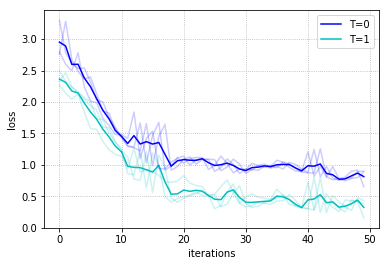
\includegraphics[width=\linewidth]{img/comp_funnel.png}
\endminipage\hfill
\minipage{0.45\textwidth}
  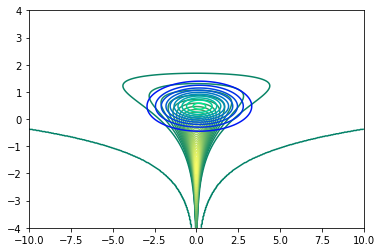
\includegraphics[width=\linewidth]{img/funnel1.png}
\endminipage
\minipage{0.45\textwidth}%
  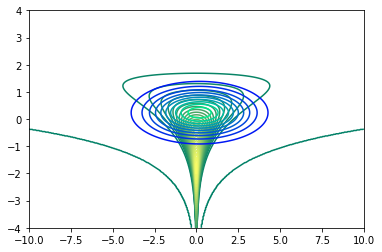
\includegraphics[width=\linewidth]{img/funnel2.png}
\endminipage
\end{center}
\caption{{\bf Top: evolution of the negative ELBO loss objective over  50 iterations. Darker lines depict mean along different seeds (lighter lines). Bottom left: contour curves (blue-turquoise) of the variational approximation with no refinement ($T=0$) at iteration 30 (loss of $1.011$). Bottom right: contour curves (blue-turquoise) of  refined variational approximation ($T=1$) at iteration 30 (loss of $0.667$). Green-yellow curves denote target density.}}\label{fig:funnel}
\end{figure}



%%%%%%%%%%%%%%%%%%%%%%%%%%%%%%
\subsection{State-space  Markov models}

We test our variational approximation on two state-space models, one for discrete data and another for continuous observations. These experiments also demonstrate that the framework is compatible with standard inference techniques such as the sum-product scheme from the Baum-Welch algorithm or Kalman filter.
In both models, we perform inference on their 
parameters $\theta$.
All the experiments in this subsection use the Fast AD version (Section \ref{sec:AD}) as it was not necessary to further tune the sampler parameters to obtain competitive results. Full model implementations can be checked in Appendix \ref{app:ss}, based on \texttt{funsor}\footnote{\url{https://github.com/pyro-ppl/funsor/}}, a PPL on top of the \texttt{Pytorch} autodiff framework.



\noindent\textbf{Hidden Markov Model (HMM)}. The model equations are 
\begin{equation}\label{snow}
p(x_{1:\tau} , z_{1:\tau}, \theta) = \prod_{t=1}^\tau p(x_t|z_t,\theta_{em})p(\bm{z_t|z_{t-1}},\theta_{tr})p(\theta),
\end{equation}
where each conditional is a Categorical distribution taking 
five different classes.  The prior is $p(\theta) = p(\theta_{em})p(\theta_{tr})$ based on two Dirichlet distributions that sample the observation and state transition probabilities, respectively. 

\noindent\textbf{Dynamic Linear Model (DLM)}. The model
equations are as in (\ref{snow}), though the conditional distributions are now Gaussian and the parameters $\theta$ refer to the observation and transition variances.  \\

 For each model, we generate a synthetic dataset, and use the refined variational approximation with $T = 0, 1, 2$. As the original variational approximation to the parameters $\theta$ we use a Dirac Delta. Performing VI with this approximation corresponds to MAP estimation using 
 the Baum-Welch algorithm in the HMM case \cite{rabiner1989tutorial} and
 the Kalman filter in the DLM case \cite{zarchan2013fundamentals},
  as we marginalize out the latent variables $z_{1:\tau}$. We use the VIS-P variant since it is {\bf sufficient  to show performance gains in this case.}%Model details are given in Appendix \ref{app:hmm}. 
 
 Figure \ref{fig:ss} shows results. The first row reports the experiments related to the HMM; the second one to the DLM. While in all graphs we report the evolution of the log-likelihood during inference, the first column reports the number of ELBO iterations, whereas the second column portrays 
 wall-clock times as the optimization takes place. They confirm that VIS ($T>0$) achieves better results than standard VI ($T=0$) for a comparable amount of time. {\bf Note also  that there is not much gain when going from $T=1$ to $T=2$ as there is from $T=0$ to $T=1$, suggesting the need to carefully 
 monitor such parameter. Finally, the top right graph for the case $T=0$ is shorter as it requires less wall-clock time.}

\begin{figure}[!htb]
\minipage{0.45\textwidth}
  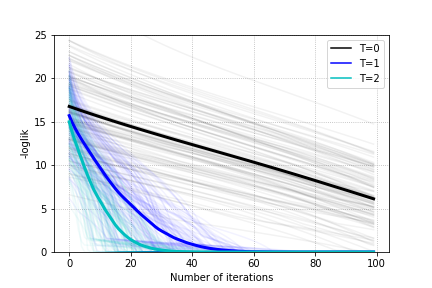
\includegraphics[width=\linewidth]{img/hmm_results.png}
\endminipage
\minipage{0.45\textwidth}
  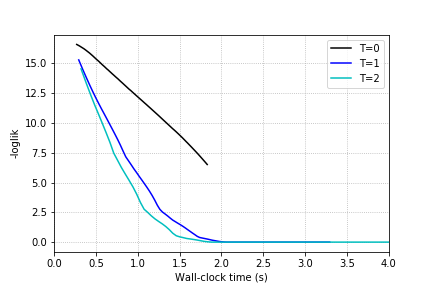
\includegraphics[width=\linewidth]{img/hmm_times.png}
\endminipage\hfill
\minipage{0.45\textwidth}%
  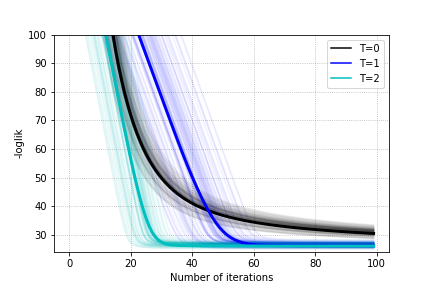
\includegraphics[width=\linewidth]{img/dlm_results.png}
 \endminipage
 \minipage{0.45\textwidth}%
  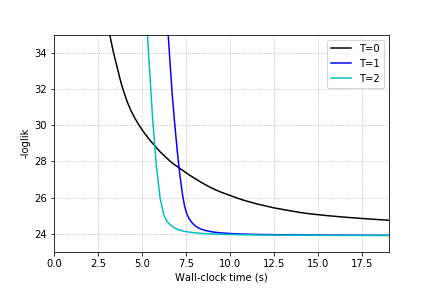
\includegraphics[width=\linewidth]{img/dlm_times.png}
\endminipage
\caption{Results of ELBO optimization for state-space models. Top left (HMM): -loglikelihood against number of ELBO gradient iterations. Top right (HMM): -loglikelihood against wall-clock time. Bottom left (DLM): -loglikelihood against number of ELBO gradient iterations. Bottom right (DLM): -loglikelihood against against wall-clock time}\label{fig:ss}
\end{figure}
    
\subsubsection{Prediction  with a HMM} 
With the aim of assessing whether ELBO optimization helps in attaining better auxiliary scores, results in a prediction task are also reported. We generate a synthetic time series of alternating 0 and 1 for $\tau=105$ timesteps. We train the previous HMM model from before on the first 100 points, and report in Table \ref{tbl:preds} the accuracy of the predictive distribution $p(y_t)$ averaged over the final 5 time-steps. We also report the predictive entropy as it helps in assessing the confidence of the model in its forecast, being a strictly proper scoring rule \cite{gneiting2007strictly}. To guarantee the same computational budget time and a fair comparison, the model without refinement is run for 50 epochs (an epoch is a full iteration over the training dataset), whereas the model with refinement is run for 20 epochs. Observe that the refined model achieves higher accuracy than its counterpart. In addition,
it is correctly more confident in its predictions.
\begin{table}[!ht]
\centering
\caption{Prediction metrics for the HMM.}\label{tbl:preds}
\begin{tabular}{lcc}
\cline{1-3}
   & $T=0$                             & $T=1$   \\ 
 \cline{1-3}
    accuracy          & $0.40$ &  $\bm{0.84}$ \\
    predictive entropy          & $1.414$ &  $\bm{1.056}$ \\
    logarithmic score   & $-1.044$ & $\bm{-0.682}$ \\
 \cline{1-3}
\end{tabular}
\end{table}

%%%%%%%%%%%%%%%%%%%%%%%%%%%%%%%%%%%%%%%
\subsubsection{Prediction with a DLM}

We test the VIS framework on the Mauna Loa monthly $CO_2$ time series data \cite{keeling2005atmospheric}. As training set, we take the first 10 years and test  over the next 2 years. We use a DLM composed of a local linear trend plus a seasonal block of periodicity 12. %Full model specification are 
%in Appendix \ref{app:ss}.
Data is standardized %As a preprocessing step, we standardize the time series 
to {\bf mean zero and standard deviation one}. To guarantee the same computational budget time, the model without refining is run for 10 epochs, whereas the model with refinement is run for 4 epochs.  Table \ref{tbl:preds_dlm}
reports the mean absolute error (MAE) and predictive entropy. 
In addition, we compute the interval score 
 \cite{gneiting2007strictly}, a strictly proper scoring rule. As can be seen, for similar wall-clock times, the refined model not only achieves lower MAE, but also its predictive intervals are narrower than the non-refined counterpart. 

\begin{table}[!ht]
\centering
\caption{Prediction metrics for the DLM.}\label{tbl:preds_dlm}
\begin{tabular}{lcc}
\cline{1-3}
   & $T=0$                             & $T=1$   \\ 
 \cline{1-3}
    MAE          & $0.270$ &  $\bm{0.239}$ \\
    predictive entropy          & $2.537$ &  $\bm{2.401}$ \\
    interval score ($\alpha=0.05$) & $15.247$ & $\bm{13.461}$\\
 \cline{1-3}
\end{tabular}
\end{table}

%%%%%%%%%%%%%%%%%%%%%%%%%%%%%
\subsection{Variational Autoencoder}

The third batch of experiments shows that VIS 
is competitive with respect to other algorithms from the recent literature including \emph{unbiased implicit variational inference} (UIVI,  \cite{pmlr-v89-titsias19a}), \emph{semi-implicit variational inference} (SIVI, \cite{yin2018semi}),  \emph{variational contrastive divergence} (VCD,  \cite{pmlr-v97-ruiz19a}), 
and the HMC variant from \cite{hoffman2017learning}, showing that our framework can outperform those approaches in similar experimental settings. 

 To this end, we test it with a Variational Autoencoder (VAE) model \cite{kingma2013auto}. %Performing efficient and flexible inference in a VAE is useful since it is the building block of more complex models and tasks \cite{chen2018symmetric,bouchacourt2018multi}. 
The VAE defines a conditional distribution $p_{\theta}(x | z)$, generating an observation $x$ from a latent variable $z$ using {\bf parameters $\theta$}. For this task, our interest 
is in modelling the $28 \times 28$ image distributions 
underlying the MNIST \cite{lecun-mnisthandwrittendigit-2010} and the fashion-MNIST \cite{xiao2017/online} datasets. To perform inference (learn
the parameters $\theta$) the VAE introduces a variational approximation $q_{\phi}(z | x)$. In the standard setting, this distribution is Gaussian; we instead use the refined variational approximation comparing various values of $T$. We used the VIS-MC approximation (though achieved similar results
with VIS-G) with the Full AD variant from Section \ref{sec:AD}.

As experimental setup, we reproduce the setting in \cite{pmlr-v89-titsias19a}. For $p_{\theta}(x | z)$, we use a factorized Bernoulli distribution parameterized by a two layer feed-forward network with 200 units in each layer and relu activations, except for a final sigmoid activation. As variational approximation $q_{\phi}(z | x)$, we use a Gaussian with mean and (diagonal) covariance matrix parameterized by
two distinct neural networks with the same structure as the previous one, except that the sigmoid activation for the mean and a softplus activation for the covariance matrix.



\begin{table}[!ht]
\centering
\caption{Test log-likelihood on binarized MNIST and fMNIST. }\label{tbl:vae}
\begin{tabular}{lcc}
\cline{1-3}
\textbf{Method}   & \textbf{MNIST}                             & \textbf{fMNIST}   \\ \cline{1-3}
 \multicolumn{3}{c}{\small Results from \cite{pmlr-v89-titsias19a}}       \\
    UIVI          & $-94.09$ &  $-110.72$ \\
    SIVI          & $-97.77$ &  $-121.53$ \\
    VAE          & $-98.29$ &  $-126.73$ \\
    \cline{1-3}
 \multicolumn{3}{c}{\small Results from \cite{pmlr-v97-ruiz19a}}       \\
    VCD          & $-95.86$ &  $-117.65$ \\
    HMC-DLGM & $-96.23$ & $-117.74$ \\ 
    \cline{1-3}
    \multicolumn{3}{c}{\small This paper}       \\
    %VIS-10-20 (this paper)     & --- & $\bm{-106.90}$  \\
    VIS-5-10     & $\bm{-82.74 \pm 0.19}$ & $\bm{-105.08 \pm 0.34}$  \\
    %VIS-0-20 (this paper)    & --- & $-121.11$  \\
    VIS-0-10     & $-96.16 \pm 0.17$ & $-120.53 \pm 0.59$  \\
    %VAE + RealNVP     & --- & ---  \\
    %VAE + IAF         & --- & --- \\
    VAE (VIS-0-0)              & $-100.91 \pm 0.16$ & $-125.57 \pm 0.63$ \\
\end{tabular}
\end{table}
%\begin{table}[!ht]
%\centering
%\caption{OLD Test log-likelihood on binarized MNIST and fMNIST.}\label{tbl:iwhvae}
%\begin{tabular}{lcc}
%\cline{1-3}
%\textbf{Method}   & \textbf{MNIST}                             & \textbf{fMNIST}   \\ \cline{1-3}
%\multicolumn{3}{c}{\small Results from \cite{pmlr-v89-titsias19a}}       \\
%    UIVI          & $-94.09$ &  $-110.72$ \\
%    SIVI          & $-97.77$ &  $-121.53$ \\
%    VAE          & $-98.29$ &  $-126.73$ \\
%    \cline{1-3}
    %VIS-10-20 (this paper)     & --- & $\bm{-106.90}$  \\
%    VIS-5-10 (this paper)     & $\bm{-82.47 \pm 0.88}$ & $\bm{-107.32 \pm 1.01}$  \\
    %VIS-0-20 (this paper)    & --- & $-121.11$  \\
%    VIS-0-10 (this paper)     & $-98.13 \pm 0.13$ & $-120.96 \pm 0.58$  \\
    %VAE + RealNVP     & --- & ---  \\
    %VAE + IAF         & --- & --- \\
%    VAE (VIS-0-0)              & $-100.92 \pm 0.09$ & $-125.88 \pm 0.62$ \\
%\end{tabular}
%\end{table}
Results are reported in Table \ref{tbl:vae}. To guarantee 
 fair comparison, we trained the VIS-5-10 variant for 10 epochs, whereas all the other variants were trained for 15 epochs (fMNIST) or 20 epochs (MNIST), so that the VAE performance is comparable to the one reported in \cite{pmlr-v89-titsias19a}. Although VIS is trained for less epochs, by increasing the number $T$ of MCMC iterations, we dramatically improve the test log-likelihood. In terms of computational complexity, the average time per epoch using $T=5$ is 10.46 s, whereas with no refinement ($T=0$) is 6.10 s (hence our decision to train the refined variant for less epochs): a moderate increase in computing time may be worth because of the dramatic increase in log-likelihood while not introducing new parameters in the model, except for the learning rate $\eta$.

Finally, as a visual inspection of the VAE reconstruction 
quality trained with VIS, Figures \ref{fig:reco} and \ref{fig:reco2} respectively display ten random samples of each dataset.
\begin{figure}[!ht]
  \begin{center}
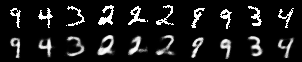
\includegraphics[width=\linewidth]{img/reco_mnist.png}
\end{center}
  \caption{Top: original images from MNIST. Bottom: reconstructed images using VIS-5-10 at 10 epochs.}\label{fig:reco}
\end{figure}

\begin{figure}[!ht]
  \begin{center}
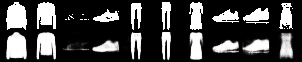
\includegraphics[width=\linewidth]{img/reconstruction_mnist_gauss8_5_10_0_.png}
\end{center}
  \caption{Top: original images from fMNIST. Bottom: reconstructed images using VIS-5-10 at 10 epochs.}\label{fig:reco2}
\end{figure}

%%%%%%%%%%%%%%%%%%%%%%%%%%%%%%%%%%%%%%%%%%%%%%%%%%%%%%%%%%
\subsection{Variational Autoencoder as a deep Bayes classifier}\label{sec:exp}
%\section{Concrete examples}
%Influence Diagrams and Probabilistic Graphical Models
With the final experiments, we show that VIS can deal with more general probabilistic graphical models, {\bf and also perform well in other inference tasks such as classification}.
%Influence diagrams \cite{howard2005influence} are popular representations of decision analysis problems, there being a long history on bridging the gap between influence diagrams and probabilistic graphical models (see \cite{doi:10.1287/opre.36.4.589}, for instance), so developing better tools for Bayesian inference can be transferred to solve influence diagrams.
We showcase the flexibility of the proposed scheme to solve inference problems in an experiment with a classification task in a high-dimensional setting, %As dataset we use the MNIST \cite{lecun1998gradient} handwritten digit classification task is chosen, in which grey-scale $28 \times 28$ images have to be classified in one of the ten classes $\mathcal{Y} = \lbrace 0, 1, \ldots, 9 \rbrace$.
with the MNIST dataset.
More concretely, we extend the VAE model conditioning it on a discrete variable $y \in \mathcal{Y} = \lbrace 0, 1, \ldots, 9 \rbrace$, leading to a conditional VAE (cVAE). The cVAE defines a decoder distribution $p_\theta(x | z, y)$ on an input space $x \in \mathbb{R}^D$ given class label $y \in \mathcal{Y}$, latent variables $z \in \mathbb{R}^d$ 
and parameters $\theta$. Figure \ref{fig:deep_bayes} depicts the corresponding {\bf probabilistic graphic model}. Additional details regarding the model architecture and hyperparameters are in Appendix
\ref{sec:detail}.

To perform inference, a variational posterior is learned as an encoder $q_\phi(z|x,y)$ from a prior $p(z) \sim \mathcal{N}(0, I)$.
Leveraging the conditional structure on $y$, we use the generative model as a classifier using Bayes rule
\begin{equation}\label{eq:mc_cvae}
p(y|x) \propto p(y)p(x|y) = p(y) \int p_\theta(x|z,y)q_\phi(z|x,y)dz  \approx  \frac{1}{M} \sum_{m=1}^M p_\theta (x | z^{(m)}, y)p(y), 
\end{equation}
where we use $M$ Monte Carlo samples $z^{(m)} \sim q_\phi(z|x,y)$. In the experiments we set $M = 5$. Given a test sample $x$, the label $\hat{y}$ with highest probability $p(y|x)$ is predicted.
%assume the existence of a data generating process, $p_{\theta}(x|z,y)$, that generates an instance $x$ belonging to class $y$ and latent variables $z$. The goal of the classifier is, given observed data $x$, predict a label $\hat{y}$ to achieve high utility $U(y, \hat{y})$. We aim at maximizing expected utility. For simplicity, as utility function we assume the standard 1-0 utility, in which $U(y, \hat{y}) = 1$ if $y = \hat{y}$ and $0$ otherwise (though other utility functions are straightforward to implement), thus promoting the classifier to achieve high classification accuracy (i.e., low classification error).
%As it is standard in the supervised learning setting, we split the dataset into a training set, used to learn the variational approximation and model parameters $\theta$, and a testing set, in which we report the mean utility achieved by the classifier for several inference strategies. As dataset, the MNIST \cite{lecun1998gradient} handwritten digit classification task is chosen, in which grey-scale $28 \times 28$ images have to be classified in one of the ten classes $\mathcal{Y} = \lbrace 0, 1, \ldots, 9 \rbrace$. 
\begin{figure}[ht]
  \begin{center}
\begin{tikzpicture}[x=1.7cm,y=1.8cm] %[x=1.7cm,y=1.8cm]
  % Nodes
\node[latent]    (Z)      {$Z$} ; %
\node[obs, below=of Z, yshift=+0.5cm]                   (X)      {$X$} ; %
 \node[latent, right=of Z]    (Y)      {$Y$} ; % 
 %\node[utility, below=of Y, yshift=+0.5cm]                   (U)      {$U$} ; %
 \node[decision, below=of X, yshift=+0.5cm]                   (Yh)      {$\hat{Y}$} ; %

%\node[const, below=of Z0, yshift=1cm]                   (mu)      {$\mu$} ; %

   \factor[below=of Z, , yshift=0.3cm]     {Z0-f}     {left:$\theta$} {Z} {X} ; %
    \factor[left=of Y, , yshift=-0.9cm]     {Y0-f}     {left:$\theta$} {Y} {X} ; %

%\edge {Z} {X};
%\edge {Y} {X};
\edge {X} {Yh};
%\edge {Y} {U};
%\edge {Yh} {U};

\end{tikzpicture}
\end{center}
  \caption{{\bf Probabilistic graphical model} for the deep Bayes classifier.}\label{fig:deep_bayes}
\end{figure}

For comparison, we perform several experiments changing $T$ in 
the transition distribution $Q_{\eta, T}$ of 
the refined variational approximation. %Note that to solve this ID, apart from learning good variational parameters,it is also required to learn sufficiently good model parameters $\theta$. Hence, the optimization problem to be solved requires alternate updates of the form
%\begin{align*}
%\phi_{t+1} = \phi_t + \lambda \nabla_{\phi} \mbox{ELBO}(q) \\
%\theta_{t+1} = \theta_t + \lambda \nabla_{\theta} \mbox{ELBO}(q).
%\end{align*}
Results are in Table \ref{tab1}, which reports
test accuracy at 
end of {\bf the refinement phase}. Note that we are comparing different values of $T$ depending on being on the {\bf refinement or inference} phases (in the latter, the model and variational parameters are kept frozen). The model with $T_{ref} = 5$ was trained for 10 epochs, whereas the other settings were for 15 epochs, to give all settings similar training time.  Results are averaged over 3 runs with different random seeds. In all settings we used the VIS-MC approximation for the entropy term. From the results, it is clear that the effect of using the refined variational approximation (the cases when $T > 0$) is crucially beneficial to achieve higher accuracy. The effect of learning a good initial distribution and inner learning rate by using the gradients $\nabla_{\phi} \mbox{ELBO}(q)$ and $\nabla_{\eta} \mbox{ELBO}(q)$ has a highly positive impact in the accuracy obtained.

On a final note, we have not included the case when only using a SGD or a SGLD sampler (i.e., without learning an initial distribution $q_{0, \phi} (z|x)$) since the results were much worse than those in Table \ref{tab1}, for a comparable computational budget. This strongly suggests that for inference in high-dimensional, continuous latent spaces, learning a good initial distribution through VIS may accelerate mixing time
dramatically.
\iffalse
\begin{table}
\caption{Results on digit classification task using deep Bayes classifier.}\label{tab1}
\centering
\begin{tabular}{llccc}
\hline
$T_{tr}$ &  $T_{te}$ & $-\mbox{ELBO}_{tr}$ & $-\mbox{ELBO}_{te}$ & $U_{te}$ (acc.) \\
\hline
0 & 0 & 113.568 & 113.551 & 95.38 \% \\ \hline
0 & 10 & 113.568 & 112.216 &  95.42 \%\\
5 & 10 & \textbf{110.370} & \textbf{109.231} &  \textbf{95.80 \%} \\ \hline
0 & 50 & 113.568 & 110.731 & 95.66 \% \\
10 & 50 & \textbf{110.879} & \textbf{107.702} &  \textbf{99.8 \pm 0.2 \%} \\
\hline
\end{tabular}
\end{table} 
\fi

\begin{table}
\caption{Results on  digit classification task using a deep Bayes classifier.}\label{tab1}
\centering
\begin{tabular}{llc}
\hline
$T_{ref}$ &  $T_{inf}$ & Acc. (test) \\
\hline
0 & 0  & $96.5 \pm 0.5$ \% \\ 
0 & 10 &  $97.7 \pm 0.7$ \%\\
5 & 10 & $ \mathbf{99.8 \pm 0.2}$ \% 
\end{tabular}
\end{table} 

\iffalse
\subsection{Gaussian Mixture Model}

See \url{http://pyro.ai/examples/gmm.html} for reference.

The model is described as (simplified version)
\begin{align*}
    w &\sim \mathcal{D}irichlet \\
    \sigma &\sim \mathcal{L}ognormal \\
    \mu_k &\sim \mathcal{N}ormal \\
    z_i &\sim \mathcal{C}ategorical(w)  \\
    x_i &\sim \mathcal{N}(\mu\left[z_i\right], \sigma) 
\end{align*}
The variational posterior is specified as $q(w, \sigma, \mu | \bm{x})$, where the discrete variables $z_i$ have been marginalized out (by using TVE in Pyro or sampling in tensorflow-probability). We compare our framework of embedding a sampler inside VI versus just using sampling or just using VI.

Now we list potential augmentations to the model that will be also tested in the experiments:
\begin{enumerate}
    \item $d \sim \mathcal{C}at(w) \rightarrow d \sim \mathcal{C}at(cw)$ (reparameterization as described in Section \ref{sec:reparam}), that should be useful in cases where the resulting $w$ is imbalanced (or there is little data for one cluster).
    \item Instead of the previous continuous reparameterization using $c$, we could add a previous $\mathcal{C}at$ sampling statement leading to the following sequence:
    \begin{align*}
        d_0 &\sim \mathcal{C}at(w_0) \\
        d &\sim \mathcal{C}at(w\left[d_0\right])
    \end{align*}
    where $w$ is now a matrix instead of a vector of probabilities.
    
    
    Benefits: can also perform exact inference since everything is discrete.
\end{enumerate}
\fi


%TODO: repeat VAE experiments using VIS-FP.

\section{CONCLUSION}
%\section{Conclusion}

We have proposed a flexible and efficient framework to perform
large-scale Bayesian inference in probabilistic models. The scheme benefits from useful properties and can be 
employed to efficiently perform inference in a wide class of models such as state space time series, variational autoencoders {\bf and variants such as the conditioned VAE for classification tasks}, defined through continuous, high-dimensional distributions.

The framework can be seen as a general 
approach to tuning MCMC sampler parameters, adapting the initial distributions and learning rate. %We believe the proposed scheme can be successfully applied to Adversarial Risk Analysis \cite{rios2009adversarial}, since MAIDs \cite{koller2003multi} are considered in that setting and it is customary to account for additional uncertainty over an attacker's influence diagram. Our framework paves the way for flexible inference and decision making under uncertainty in these settings, and we will explore this in future work.
Key to the success and applicability of the VIS framework are the ELBO approximations based on the refined variational approximation introduced, which are computationally cheap but convenient. 

Better estimates of the refined density and its gradient may be a fruitful line of research, such as the spectral estimator from \cite{shi2018spectral}. Another alternative is to use a deterministic flow (such as SGD or SVGD), keeping
track of the change in entropy at each iteration using the change of variable formula as  in \cite{duvenaud2016early}. However, this requires a costly Jacobian computation, making it unfeasible to combine with our \emph{backpropagation through the sampler} scheme (Sec. \ref{sec:tuning}) for moderately complex problems. We leave this for future exploration. {\bf Another interesting and useful line for further action would be to tackle the case where the latent variables $z$ are discrete. This would entail adapting the automatic differentiation techniques to be able to backpropagate the gradients through the sequences of acceptance steps necessary in Metropolis-Hastings samplers.}

Of independent interest to deal with the implicit variational density, it may be worthwhile to consider optimizing the Fenchel dual of the KL divergence, as
 in \cite{fang2019implicit}. However, this requires the use of an auxiliary neural network, which may entail a large computational price to pay compared with our lighter particle approximation.


Lastly, probabilistic programming offers powerful tools for Bayesian modelling.
A PPL can be viewed as a programming language extended with random sampling and Bayesian conditioning capabilities, complemented with an inference engine that produces answers to inference, prediction and decision making queries. Examples 
include  WinBUGS \cite{lunn2000winbugs}, Stan \cite{carpenter2017stan}, or the recent Edward \cite{tran2018simple} and Pyro \cite{bingham2018pyro}. We plan to adapt VIS into several PPLs to ease the adoption of the framework.


\section{SG-MCMC}

\subsection{Further ideas}

Approximate the $\mathcal{O}(n^2)$ attention matrix with the sum of global attention, local attention and random attention, as in Big Bird.

Think about how to frame the sliding window for local attention since in this case we are dealing with particles instead of tokens from textual data. Instead of banded matrix (sliding window), we can use a block diagonal matrix (particles are assigned to groups, which can be fixed or dynamic).






